\chapter{User Manual}
\label{ch:usermanual}

	\section{Welcome}
	\label{sec:welcome}

		\begin{wrapfigure}{R}{0.25\textwidth}
			\vspace{-5em}
			\centering
			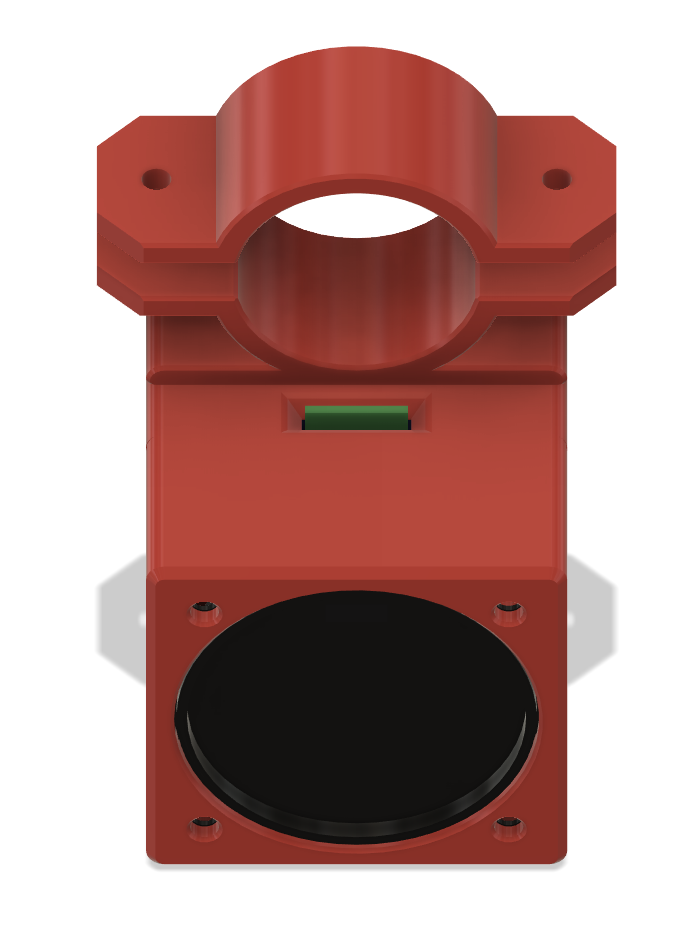
\includegraphics[width=0.25\textwidth]{graphics/final-cad.png}
		\end{wrapfigure}

		The Walking Aid Usage Prompt System is a medical aid consisting of a pair of hardware devices that allows patients suffering with dementia to be automatically reminded to use their walking aid when they begin walking without it. With stastically high rates of falling in dementia patients, the Walking Aid Usage Prompt System attempts to reduce these numbers. It aims to do this by offering a system that automatically detects when patients are walking without their walking aid and plays them a reminder to take their walking aid with them.

		\paragraph{Automatic Movement Detection}\mbox{}

		With the use of an accelerometer in each device, our systems can automatically detect when your patient is moving, and if they are moving without their walking aid.

		\paragraph{Remind the patient with the sound of a familiar voice}\mbox{}

		Utilising the SD card reader on the walking aid device, you can upload an MP3 file to be played to the patient when they begin walking without their walking aid. The connected speaker will give you the peace of mind that the patient will hear the reminder whenever it needs to be played.

		\begin{wrapfigure}{L}{0.25\textwidth}
			\vspace{-1em}
			\centering
			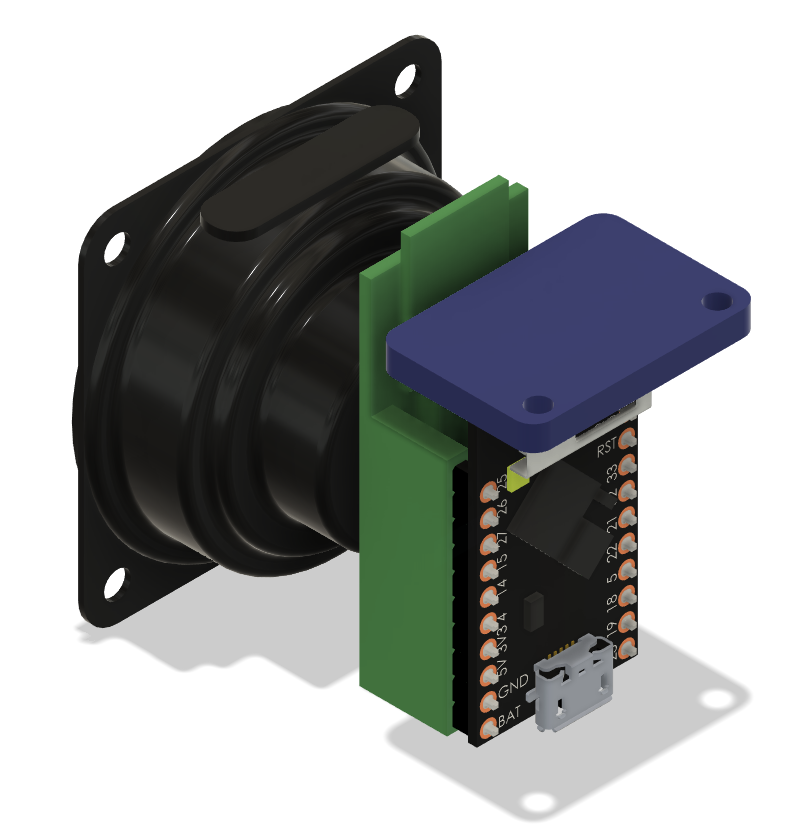
\includegraphics[width=0.25\textwidth]{graphics/hardware.png}
		\end{wrapfigure}

		\paragraph{Use a vibration reminder for patients who are hard of hearing}\mbox{}

		The inclusion of a communication protocol between our two devices will mean that the use of an audio reminder can be replaced, with the wearable device being asked to vibrate instead.

		\paragraph{Never use intrusive wearables again}\mbox{}

		Boasting a small form factor and the avoidance of distracting LEDs, our devices were developed with the comfort of the patient in mind. Utilising 18mm x 32mm TinyPICO development boards, our solution manages to keep device sizes to a minimum and can be worn on either the ankle or the wrist. 

		\paragraph{Next Steps:}\mbox{}

		\vspace{1em}
		Excited to get started?

		\textit{\hyperref[sec:quick_start_guide]{Click here for our Quick Start Guide} or head to section \ref{sec:quick_start_guide}}

		\vspace{1em}
		Want to learn more?

		\textit{\hyperref[sec:user_guide]{Click here for our more in depth User Guide} or head to section \ref{sec:user_guide}}

		\vspace{1em}
		Are you a developer?

		\textit{\hyperref[sec:developer_guide]{Click here to head to our developer guide} or head to section \ref{sec:developer_guide}}

	\newpage
	\section{Quick Start Guide}
	\label{sec:quick_start_guide}

		\subsection{Introduction}
		\label{subsec:quick_start_guide_introduction}

			The Walking Aid Usage Prompt system is a medical aid that allows patients to be automatically reminded to use their walking aid when they begin walking without it. The whole system comprises of two separate devices, one to be attached to the user's walking aid and the other to the ankle or wrist of the user. The wearable device is used to detect when the user has taken 5 steps within a 10 second period to signify that the user has began walking. Once this occurs, the wearable device communicates with the user's walking aid device to make a check to see if the walking aid is moving also. If the walking aid is moving, then great! There is no need to worry, the user is making use of their walking aid. However, should a user not be utilising their walking aid, then the walking aid can either play an audio reminder to the user, or it can communicate back to the wearable device to vibrate against the ankle or the wrist of the user. Both solutions are designed to remind the user to take their walking aid with them when walking in an attempt to reduce fall rates in dementia patients.

			The remainder of this quick start guide will explain the prerequisites to ensure that the system is fully functional, and a brief setup guide so that the user can get started.

		\subsection{Hardware Requirements}
		\label{subsec:quick_start_guide_hardware}

			\paragraph{To use the audio reminder system:}\mbox{}

			\begin{itemize}
				\item MicroSD Card >= 2MB Capacity.
				\item Windows/MacOS/Linux Computer System.
				\item A means to read/write to the SD card from the computer system. For example, a USB to MicroSD card reader.
				\item A microphone to record audio.
			\end{itemize}

			\paragraph{To use the vibration reminder system:}\mbox{}

			No hardware necessary, please advance to section \ref{subsec:quick_start_setup_guide}.

		\subsection{Software Requirements}
		\label{subsec:quick_start_guide_software}

			\paragraph{To use the audio reminder system:}\mbox{}

			\begin{itemize}
				\item Voice recording software such as Windows Voice Recorder or Audacity. (An alternative could be to record your voice message on a mobile device and transfer it to your computer system).
				\item File explorer software to copy the file to the SD card.
				\item MP3 audio file should be <= 2MB in size.
			\end{itemize}

			\paragraph{To use the vibration reminder system:}\mbox{}

			No software necessary, please advance to section \ref{subsec:quick_start_setup_guide}.

		\subsection{Setup Guide}
		\label{subsec:quick_start_setup_guide}
			

	\section{User Guide}
	\label{sec:user_guide}

	\section{Developer Guide}
	\label{sec:developer_guide}

	% \section{Introduction}
	% \label{sec:usermanual_intro}

	% 	Intro on what the devices to, prerequisites, etc

	% 	\todo{We probably need health disclaimers somewhere in our doc?}

	
	% \section{Hardware Guide}
	% \label{sec:usermanual_hardware}

	% 	Hardware stuff, powering on device, inserting sd card, assembly/dissasmbly guide? 

	% \section{Software Guide}
	% \label{sec:usermanual_software}

	% 	Software related things, setting device up with voice recording on sd card etc?


	% \section{Development Guide}
	% \label{sec:usermanual_development}

	% 	Code related guide
